\subsection{Knot inference}

%In many problems, the quantities of main interest are change-points or break-points in the model, such as change-points detection in time series \citep{aminikhanghahi2017survey,truong2020selective}. Thus researchers want to construct an accurate estimation for change-points with rigorous statistical approaches \citep{doi:10.1080/01621459.2015.1073154,doi:10.1080/01621459.2021.1947307}. 
We perform EBARS for knot inference in linear spline regression. % The linear spline is a piecewise linear model. 
Line segments are connected in unique knots and the spline is discontinuous at the location where two knots coincide. The data is generated from three linear spline models with one, two and four knots as shown in Figure \ref{fig:knot_estimation}, where the knot locations are respectively $(0.5),~(0.3,0.7),~(0.2,0.2,0.5,0.7)$. The functions are continuous except for the spline with $k=4$. The noise is Gaussian with standard deviation $0.4$, $0.3$, $0.4$. 

\begin{figure}
    \centering
    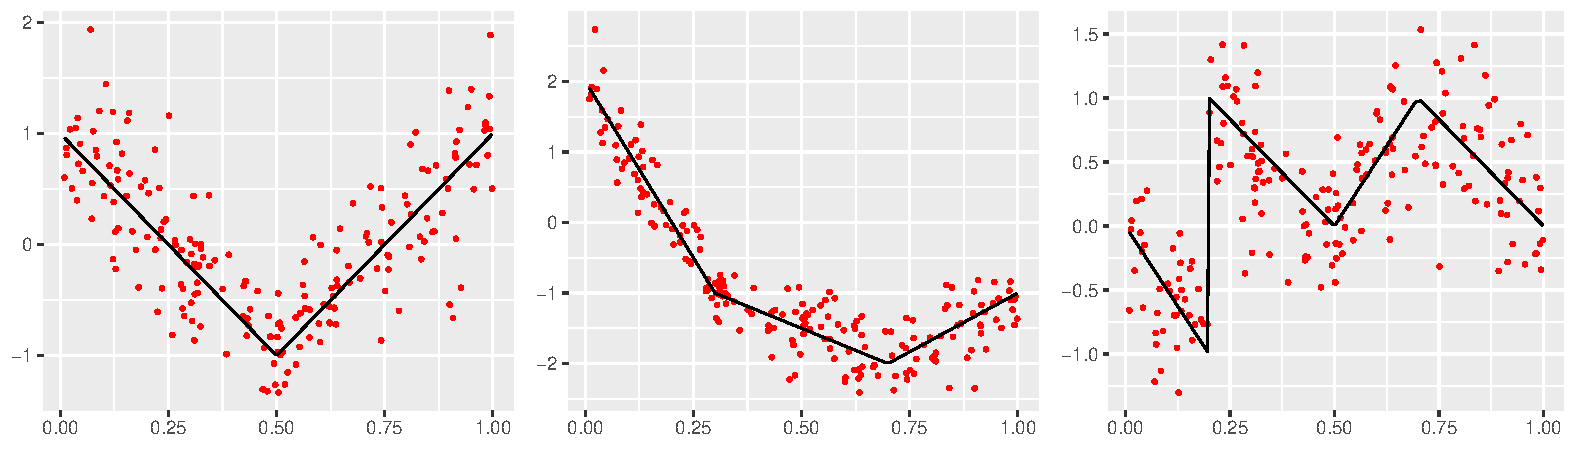
\includegraphics[width=0.9\textwidth]{Experiments/plots/knot_estimation.pdf}
    \caption{Linear splines with one, two and four knots. Black segments are true spline curves and red points are noisy observed data with $m=200$.}
    \label{fig:knot_estimation}
\end{figure}

Figure \ref{fig:knot_inference} illustrates the posterior distribution of the knot number and location by EBARS with $\gamma=1$ in $k=1,2,4$. The sample size is $500$ in all scenarios. We simulate $5000$ samples of $(k,\xi)$ via RJMCMC after $5000$ burning steps. Histograms show that the average knot number is close to the true value with negligible error. From the density plots, the posterior mass concentrates on the correct location of change points in all cases even though the knot number is unknown. Especially, for $k=4$, the posterior density at $0.2$ is double at $0.5$ and $0.7$, meaning that $0.2$ is chosen as the knot twice.

\begin{figure}
    \centering
    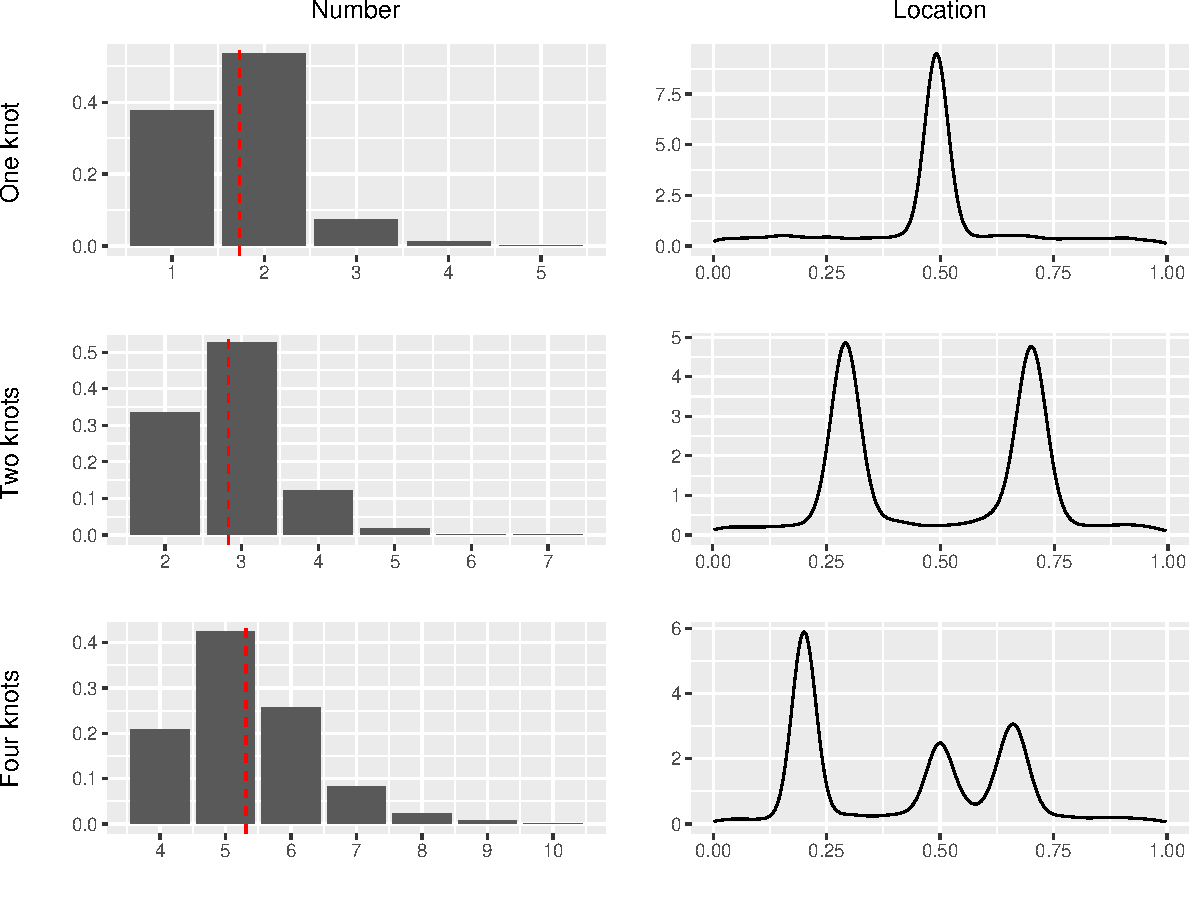
\includegraphics[width=0.9\textwidth]{Experiments/plots/knot_inference.pdf}
    \caption{The posterior distributions of knots in three scenarios by EBARS. Left channels are the histograms of the knot number, where red dashed vertical lines indicate the mean number. Right channels are the posterior density plots of the knot location.}
    \label{fig:knot_inference}
\end{figure}

To evaluate the performance of knot inference, we compare EBARS with Segmented of Muggeo and MML of Guangyu Yang and Zhang. In this experiment, the knot number is given since Segmented and MML cannot estimate $k$. The absolute error of knot location is calculated as criteria. Three methods are evaluated under sample sizes $m=200,500$ and the experiment is repeated $50$ times.

Simulation results of the mean and standard deviation of absolute errors are summarized in Tables \ref{tab:knot_1} and \ref{tab:knot_2}. When $k=1,2$, three methods obtain fairly small absolute errors. However, when $k=4$, the absolute errors of EBARS are much less than other two algorithms for all knots. MML struggles to estimate the duplicate knots $0.2$ and causes horrible bias. Segmented outperforms MML but it is still much less accurate than EBARS. Compared with MML and Segmented, our EBARS is robust and attain a precise estimation with jumping discontinuity and increasing number of knots. Furthermore, MML and Segmented are exclusively applied in linear splines and they require the knot number to be given, whereas EBARS is convenient to estimate the knot number and location simultaneously in splines of any degree.

% In this subsection, we perform EBARS for knot inference in linear spline regression given the knot number $k$. The linear spline is a piecewise linear model. Line segments are connected in unique knots and the spline is discontinuous at the location where two knots coincide. Furthermore, since $k$ is fixed, relocation becomes the only possible movement strategy in MCMC. Consequently, $\gamma$ has no effect on EBARS in this example. We compare its performance with Segmented and MML.
%Notably, their approaches are frequentist whereas EBARS is Bayesian.

% The simulation data are generated from three linear spline population models with one, two and four knots as shown in Figure \ref{fig:knot_estimation}. The knot locations are respectively $(0.5),~(0.3,0.7),~(0.2,0.2,0.5,0.7)$.  %We refer to them as Cases $2.1-2.3$. 

% The functions are continuous except for the spline with $k=4$ at $0.2$. The noise is Gaussian with standard deviation $0.4$, $0.3$, $0.4$. All methods are evaluated under sample sizes $m=200,500$ and the experiment is repeated $50$ times in each setting. Assuming that the $i$-th knot is $\xi_i$ and the estimation is $\hat{\xi}_i$, we calculate the absolute error $|\xi_i-\hat{\xi}_i|$ for each knot. 


% Simulation results are summarized in Tables \ref{tab:knot_1} and \ref{tab:knot_2}. When $k=1,2$, MML and Segmented perform slightly better than EBARS and all three methods obtain fairly small absolute errors. However, when $k=4$, the absolute errors of EBARS are much less than other algorithms for all knots. MML struggles to estimate the duplicate knots $0.2$ and causes horrible errors. Segmented outperforms MML but it is still much less accurate than EBARS. This means that our EBARS is robust and attain a precise estimation with jumping discontinuity and increasing number of knots.

% Furthermore, the MML and segmented methods are exclusively applied in linear spline models. In contrast, EBARS can handle splines of any degree with ease. Moreover, we can estimate the number and locations of knots meanwhile in EBARS, whereas MML and Segmented require $k$ to be given. This is especially important when $k$ is also of interest. Although the computational time of EBARS is relatively longer due to MCMC, EBARS is in favor if speed is not the main concern. 

\begin{table}
\caption{Absolute errors for knot location estimation of three methods in $k=1,2$}
\label{tab:knot_1}
\centering
\begin{tabular}{ccccc}
\toprule
\multirow{2}{*}{Methods} & \multirow{2}{*}{m}   & One knot       & \multicolumn{2}{c}{Two knots}    \\
\cline{3-5}
                         &                      & Knot $1$         & Knot 1         & Knot 2         \\
                         \midrule
EBARS                    & \multirow{3}{*}{200} & 0.0219(0.0126) & 0.0167(0.0150)  & 0.0248(0.0257) \\
MML                      &                      & 0.0163(0.0099) & 0.0138(0.0118) & 0.0170(0.0214)  \\
Segmented                &                      & 0.0159(0.0102) & 0.0117(0.0113) & 0.0186(0.0204) \\
\midrule
EBARS                    & \multirow{3}{*}{500} & 0.0100(0.0076)  & 0.0095(0.0065) & 0.0142(0.0122) \\
MML                      &                      & 0.0075(0.0060)  & 0.0068(0.0058) & 0.0102(0.0076) \\
Segmented                &                      & 0.0079(0.0061) & 0.0070(0.0059)  & 0.0113(0.0081) \\
\bottomrule


\end{tabular}
\end{table}

\begin{table}
\caption{Absolute errors for knot location estimation of three methods in $k=4$}
\label{tab:knot_2}
\centering
\begin{tabular}{cccccc}
\toprule
\multirow{2}{*}{Methods} & \multirow{2}{*}{m}   & \multicolumn{4}{c}{Four knots}                                      \\
\cline{3-6}
                         &                      & Knot 1         & Knot 2         & Knot 3         & Knot 4         \\
                         \midrule
EBARS                    & \multirow{3}{*}{200} & 0.0058(0.0060) & 0.0044(0.0043) & 0.0206(0.0199) & 0.0170(0.0096) \\
MML                      &                      & 0.3437(1.1010) & 0.1163(0.1283) & 0.0978(0.1006) & 0.1012(0.1454) \\
Segmented                &                      & 0.0366(0.0494) & 0.0712(0.1067) & 0.0799(0.0889) & 0.0752(0.0805) \\
\midrule
EBARS                    & \multirow{3}{*}{500} & 0.0025(0.0029) & 0.0026(0.0025) & 0.0194(0.0172) & 0.0150(0.0137) \\
MML                      &                      & 0.2737(0.4266) & 0.1725(0.1683) & 0.1065(0.1800) & 0.2131(0.5211) \\
Segmented                &                      & 0.0171(0.0346) & 0.0283(0.0775) & 0.0395(0.0825) & 0.0349(0.0805) \\
\bottomrule
\end{tabular}
\end{table}